\documentclass{BeamerTemplate}

\title{Module 7 - Intervalles de confiance}

\graphicspath{{Images/Module 7/}}

\begin{document}
\begin{frame}[t]
  \titlepage
\end{frame}

%-------------------------------------------------------------------------------------------------------------------------------------





%%%%%%%%%%%%%%%%%%%%%%%%%%%%%%%%%%%
%%%%%%%%%%%%%%%%%%%%%%%%%%%%%%%%%%%
%%%%%%%%%%%%%%%%%%%%%%%%%%%%%%%%%%%
\section{Introduction aux intervalles de confiance}


\begin{frame}[t]{Introduction: estimation ponctuelle imparfaite}

Un échantillon donne lieu à UNE estimation du paramètre. Quelle confiance peut-on avoir en cette estimation?

\vspace{2cm}
\href{https://019fb413-fe96-cbb6-5ac0-463b16f01668.share.connect.posit.cloud/}{Illustration.}

\end{frame}


\begin{frame}[t]
 \frametitle{Concept d'estimation par intervalle de confiance}

Un intervalle de confiance :
\medskip

    \begin{itemize}\itemsep8mm
    \item complète l'estimation ponctuelle en l'entourant d'une \alert{marge d'erreur}.

    \item donne une idée de la précision obtenue avec l'échantillon.

    \item est associé à un \alert{niveau de confiance} (probabilité que l'intervalle contienne la vraie valeur du paramètre).
    \end{itemize}
%\uncover<2->{
%\underline{\bf Exemple:}
%Un analyste annonce, après avoir pris un échantillon, que 76\% des étudiants en informatique trouvent un emploi juste après leur formation, avec une marge d’erreur de 0.03 et avec un niveau de confiance de 95\%.
%}
\end{frame}

%\begin{frame}[t]
% \frametitle{Interprétation}
%
%On dit que $[0.76 - 0.03, 0.76 + 0.03]$ est un intervalle de confiance de niveau 95\% pour $p$, la proportion (inconnue) des étudiants en informatique qui trouvent un emploi.
%
%\medskip
%\underline{\bf Interprétation:}
%Si on répète la m\^eme expérience un grand nombre de fois, l'intervalle de confiance contiendra la vraie valeur de $p$ dans 95\% des fois.
%\end{frame}


\begin{frame}[t]
 \frametitle{Définition formelle}

 \begin{itemize}
\item $X_1,\ldots,X_n$:  échantillon aléatoire de taille $n$;
\item $\theta$:  paramètre d'intér\^et (comme $\mu$ ou $\sigma^2$);
 \end{itemize}
 \begin{Boite}{Intervalle de confiance de niveau $1-\alpha$ pour un paramètre $\theta$}
 {Deux statistiques  $[C_1, C_2]$ telles que  \alert{$$P(C_1\le \theta\le C_2)=1-\alpha$$}
}
 \end{Boite}


 \medskip
 \uncover<2->{
 \begin{itemize}
\item $1-\alpha$: niveau de confiance de l'intervalle \\(fixé arbitrairement par le chercheur).
\item Souvent $1-\alpha=0,95$. Parfois $1-\alpha=0,90$ ou $0,99$ ou autre.
 \end{itemize}
 }
\end{frame}


\begin{frame}{Intervalles de confiance à 95\%}
\begin{columns}[c]

  \column{0.4\textwidth}
  \begin{Boite}{\faInfoCircle\ Interprétation}
  En moyenne, 95\% des intervalles de confiance à 95\% \textbf{contiennent} la vraie valeur du paramètre.
  \end{Boite}



  \column{0.6\textwidth}
  \begin{tikzpicture}[x=6cm, y=0.6cm]
    \draw[blue, thick] (0.5, -1) -- (0.5, 9) node[pos=1.05, text=black] {\scriptsize Vraie valeur $\theta$};

    % Génération de 9 intervalles IC avec quelques non-couvrants
    \foreach \i/\a/\b/\cover in {
      0/0.3/0.7/1,
      1/0.2/0.9/1,
      2/0.1/0.6/1,
      3/0.55/0.9/1,
      4/0.4/0.65/1,
      5/0.05/0.35/0,
      6/0.2/0.6/1,
      7/0.1/0.4/0,
      8/0.3/0.8/1
    } {
      \ifnum\cover=1
        \draw[green, thick] (\a, \i) -- (\b, \i);
        \node[right, green] at (\b, \i) {\checkmark};

      \else
        \draw[red, thick] (\a, \i) -- (\b, \i);
        \node[right, red] at (\b, \i) {\faTimes};
      \fi
    }
  \end{tikzpicture}
\end{columns}

\vspace{1em}
\begin{center}
\scriptsize
\textcolor{green}{\checkmark} : l’intervalle contient $\theta$ 

\textcolor{red}{\faTimes} : l’intervalle ne contient pas $\theta$

\end{center}

\end{frame}




\begin{frame}{Rappel sur les lois échantillonnales}

 Lorsque $X_1, ..., X_n$ i.i.d. $\mathcal{N}(\mu, \sigma^2)$, on connaît les lois échantillonnales des statistiques suivantes:

\begin{center}
{\renewcommand{\arraystretch}{2.5}
\begin{tabular}{|c|l|}
\hline Statistique & Loi échantillonnale % &Espérance& Variance 
\\[-0.15cm]
\hline \hline
$\displaystyle Z=\frac{\overline X -\mu }{\sigma/\sqrt{n}}$ & \\\hline
$\displaystyle T=\frac{\overline X -\mu }{S/\sqrt{n}}$ &\\\hline
%$X_1, ..., X_n$ i.i.d. loi quelconque &
%$\displaystyle Z_*=\frac{\overline X -\mu }{S/\sqrt{n}}\approx \hspace{1cm}$ &\\[-0.5cm]
%$\mu$ et $\sigma^2$ inconnues, $n$ grand & &
$\displaystyle U=\frac{(n-1)S^2 }{\sigma^2}$ &\\\hline
\end{tabular}
}
\end{center}

 \vspace{1cm}

\end{frame}
%%%%%%%%%%%%%%%%%%%%%%%%%%%%%%%%%%%%%%%%%%%%%%%%%%%%%%%%%%%%%%%%%%%%%%%%%%%%%%%%%%%%%%%%%%%%%%%%%%%%%%%%%%%%%%%%%%%%%%%%%%%
\begin{frame}[t]{4 cas étudiés}

Nous construirons 4 intervalles de confiance:
\vspace{0.5cm}

\begin{tabular}{|c|c|l|}
  \hline
  Cas&Paramètre & Situation \\\hline
&&\\[-0.3cm]
1&  $\mu$ & $X_1, ..., X_n\;\sim\;\mathcal{N}(\mu, \, \sigma^2)$ avec $\sigma^2$ connue \\
&&\\
2&  $\mu$ & $X_1, ..., X_n\;\sim\;\mathcal{N}(\mu, \, \sigma^2)$ avec $\sigma^2$ inconnue  \\
&&\\
3&  $\mu$ & $X_1, ..., X_n\;\sim\;$ loi inconnue, mais $n$ est grand  \\[0.2cm]\hline
&&\\[-0.3cm]
4&  $\sigma^2$ & $X_1, ..., X_n\;\sim\;\mathcal{N}(\mu, \, \sigma^2)$ \\[0.2cm]\hline
%&&\\[-0.3cm]
%5&  $p$ & $X_1, ..., X_n\;\sim\;$Bernoulli($p$) et $n$ est grand \\[0.2cm]\hline
\end{tabular}
\end{frame}

%%%%%%%%%%%%%%%%%%%%%%%%%%%%%%%%%%%%%%%%%%%%%%%%%%%%%%%%%%%%%%%%%%%%%%%%%%%%%%%%%%%%%%%%%%%%%%%%%%%%%%%%%%%%%%%%%%%%%%%%%%%

\begin{comment}
png("N.png",height=3,width=5,units="in",res=100)
par(mar=c(2,0,1,1))
curve(dnorm(x,0,1), from=-4.2, to=4.2, , xlab="x",  ylab=" ",ylim=c(0,0.42),col=1,lwd=2,yaxs="i",bty="l",col.axis="white",xaxp=c(-1.64,1.64,2),xlim=c(-4,4))
mtext(0,side=1,at=0,line=1)
mtext(expressio\mathcal{N}(z[alpha/2]),side=1,at=1.64,line=1,cex=1.3)
mtext(expressio\mathcal{N}(-z[alpha/2]),side=1,at=-1.64,line=1,cex=1.3)
polygo\mathcal{N}(c(-4,seq(-4,-1.64,0.01),-1.64),c(0,dnorm(seq(-4,-1.64,0.01),),0),col="skyblue")
polygo\mathcal{N}(c(1.64,seq(1.64,4,0.01),4),c(0,dnorm(seq(1.64,4,0.01)),0),col="skyblue")
text(expressio\mathcal{N}(1-alpha),x=0,y=0.2,cex=1.5)
text(expressio\mathcal{N}(alpha/2),x=-2,y=0.02,cex=1.2)
text(expressio\mathcal{N}(alpha/2),x=2,y=0.02,cex=1.2)
dev.off()

png("t.png",height=3,width=5,units="in",res=100)
par(mar=c(2,0,1,1))
curve(dt(x,4), from=-4.2, to=4.2, , xlab="x",  ylab=" ",ylim=c(0,0.42),col=1,lwd=2,yaxs="i",bty="l",col.axis="white",xaxp=c(-2.13,2.13,2),xlim=c(-4,4))
mtext(0,side=1,at=0,line=1)
mtext(expressio\mathcal{N}(t[paste(alpha/2,"; v")]),side=1,at=2.13,line=1,cex=1.3)
mtext(expressio\mathcal{N}(-t[paste(alpha/2,"; v")]),side=1,at=-2.13,line=1,cex=1.3)
polygo\mathcal{N}(c(-5,seq(-5,-2.13,0.01),-2.13),c(0,dt(seq(-5,-2.13,0.01),4),0),col="violet")
polygo\mathcal{N}(c(2.13,seq(2.13,5,0.01),4),c(0,dt(seq(2.13,5,0.01),4),0),col="violet")
text(expressio\mathcal{N}(1-alpha),x=0,y=0.2,cex=1.5)
text(expressio\mathcal{N}(alpha/2),x=-2.5,y=0.02,cex=1.2)
text(expressio\mathcal{N}(alpha/2),x=2.5,y=0.02,cex=1.2)
dev.off()

png("K.png",height=3,width=5,units="in",res=100)
par(mar=c(2,0,1,1))
curve(dchisq(x,4), from=0, to=14, , xlab="x", ylab=" ",ylim=c(0,0.2),col=1,lwd=2,yaxs="i",bty="l",col.axis="white",xaxp=c(0,4,1),xlim=c(0,13))
axis(side=1,at=c(0,0.71,4,9.49),labels=c(0,"","v",expressio\mathcal{N}(chi[paste(alpha/2,"; v")]^2)))
mtext(expressio\mathcal{N}(chi[paste(1-alpha/2,"; v")]^2),side=1,at=1,line=1)
polygo\mathcal{N}(c(0,seq(0,0.71,0.01),0.71),c(0,dchisq(seq(0,0.71,0.01),4),0),col="salmon")
polygo\mathcal{N}(c(9.49,seq(9.49,14,0.01),14),c(0,dchisq(seq(9.49,14,0.01),4),0),col="salmon")
text(expressio\mathcal{N}(1-alpha),x=3,y=0.1,cex=1.5)
text(expressio\mathcal{N}(alpha/2),x=0.4,y=0.01,cex=1)
text(expressio\mathcal{N}(alpha/2),x=10,y=0.01,cex=1)
dev.off()
\end{comment}
\section[IC pour une moyenne]{Intervalles de confiance pour une moyenne}

\subsection{Loi normale, variance connue}

\begin{frame}[t]
 \frametitle{Cas 1 pour $\mu$: loi normale, variance CONNUE}

\small
\begin{itemize} \itemsep1mm
\item {\color{blue}{On suppose que $X_1,\ldots,X_n$ i.i.d. loi $\mathcal{N}(\mu,\sigma^2)$, \\
o\`u $\sigma^2$ est  une valeur connue}.}% et $\mu$ est le paramètre d'intér\^et.
\item On déduit que $\overline X\;\sim\;\mathcal{N}\left(\mu,\displaystyle\frac{\sigma^2}{n}\right)$, donc que    $\displaystyle Z=\frac{\overline X-\mu}{\sigma/\sqrt{n}}\;\sim\;\mathcal{N}(0,1)$
\item Soit $z_{\alpha/2}$, la valeur telle que $P(Z>z_{\alpha/2})=\alpha/2$. On a donc que\\
\end{itemize}

\vspace{-0.5cm}
$$P(\,-z_{\alpha/2}\;\le \;Z\;\le \;z_{\alpha/2}\,)=1-\alpha.$$

\begin{center}

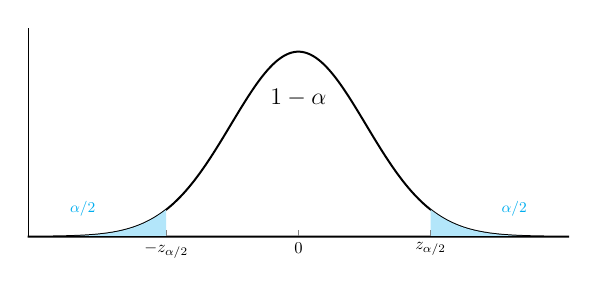
\begin{tikzpicture}[scale = 0.6]
  \begin{axis}[
    no markers,
    domain=-4:4,
    samples=200,
    axis lines*=left,
    ymin=0, ymax=0.45,
    xtick={-1.96, 0, 1.96},
    xticklabels={$-z_{\alpha/2}$, $0$, $z_{\alpha/2}$},
    ytick=\empty,
    enlargelimits=false,
    clip=false,
    axis on top,
    width=13cm,
    height=6cm
  ]

  % Courbe normale standard
  \addplot[very thick, black] {exp(-x^2/2)/sqrt(2*pi)} \closedcycle;

  % Remplissage à gauche
  \addplot [
    domain=-4:-1.96,
    samples=100,
    fill=cyan!30,
    draw=none
  ] {exp(-x^2/2)/sqrt(2*pi)} \closedcycle;

  % Remplissage à droite
  \addplot [
    domain=1.96:4,
    samples=100,
    fill=cyan!30,
    draw=none
  ] {exp(-x^2/2)/sqrt(2*pi)} \closedcycle;

  % Texte 1 - alpha
  \node at (axis cs:0,0.3) {\Large $1 - \alpha$};

  % Texte alpha/2 à gauche
  \node at (axis cs:-3.2,0.06) [cyan] {\small $\alpha/2$};

  % Texte alpha/2 à droite
  \node at (axis cs:3.2,0.06) [cyan] {\small $\alpha/2$};

  \end{axis}
\end{tikzpicture}
    
\end{center}

\end{frame}


\begin{frame}[t]
 \frametitle{Cas 1 pour $\mu$: loi normale, variance connue}

\begin{itemize} \itemsep3mm
\item On cherche $[C_1, C_2]$ tels que $P(C_1\le \alert{\mu} \le C_2)=1-\alpha$
\item On sait que $P\left(\,-z_{\alpha/2}\;\le \;\dfrac{\overline X - \mu}{\sigma/\sqrt{n}}\;\le \;z_{\alpha/2}\,\right)=1-\alpha$
\end{itemize}

\end{frame}
\begin{comment}
\begin{frame}[t]
 \frametitle{Marge d'erreur}

 \begin{itemize}
  \item Soit $\hat{\theta}$, une estimation ponctuelle de $\theta$ \\(comme $\overline x$ qui estime $\mu$)
  \item Soit $[C_1,C_2]$,  un intervalle de confiance pour $\theta$.
  \item     On dit que l'intervalle est \alert{symétrique}  s'il est de la forme $[\hat{\theta}-M,\hat{\theta}+M]$. Dans ce cas, on appelle $M$ la \alert{marge d'erreur}.

  \medskip
 \item  La \alert{longueur} d'un intervalle de confiance $[C_1,C_2]$
  est $L=C_2-C_1$. Dans le cas d'intervalles symétriques,
  $L=2M$.

  \medskip
  \item Habituellement, on choisit $C_1$ et $C_2$ de sorte que l'on
  a bien une probabilité de couverture $1-\alpha$ et pour minimiser $L$.
  \end{itemize}
\end{frame}
\end{comment}
\begin{frame}[t] \frametitle{Exemple 1 }

 {\small
 Soit $X$, le diamètre (en cm)  des disques de frein  produits par une machine, o\`u $X\sim \mathcal{N}(\mu,\, 0,0009)$.  On choisit un échantillon de 9 disques  au hasard et on calcule un diamètre moyen de $\overline{x}$ cm.

 \vspace{3mm}

 \alert{a)} Donnez un intervalle de confiance de niveau 95\% pour $\mu$. 
 }
 
 \vspace{4.5cm}
\href{https://019fb414-9ff8-69d8-4913-061353a9ec80.share.connect.posit.cloud/}{Illustration}
 
\end{frame}


\begin{frame}[t] \frametitle{Exemple 1 }

 {\small


 \alert{b)} Donnez l'IC si $\overline{x}=12,05$. 
 }
\end{frame}


\begin{frame}[t]{ }

\centerline{\LARGE\bf \alert{QUIZ !}}
\medskip
Déterminez si les énoncés suivants (liés à l'exemple 1) sont vrais ou faux.

\begin{itemize} \itemsep7mm
\item 95\% des disques de cette compagnie ont un diamètre entre 12,03 et 12,07 cm. \href{https://019fb415-41be-2c85-6b6f-3caffeb39206.share.connect.posit.cloud/}{Illustration}
\item 95\% des intervalles calculés avec cette formule (à partir d'échantillons différents) contiendraient le vrai diamètre moyen.
\item On a confiance à 95\% que l'intervalle (12,03, 12,07) cm contient la vraie valeur de $\mu$.
\item Si on prenait un nouvel échantillon de taille $n=9$, la probabilité que sa moyenne $\overline X$ soit entre 12,03 et 12,07 cm est de 95\%. \href{https://019fb415-41be-2c85-6b6f-3caffeb39206.share.connect.posit.cloud/}{Illustration}
\end{itemize}

\end{frame}

% \begin{frame}[t] \frametitle{Exemple 1: taille d'échantillon}

%  \alert{b)} Quelle taille d'échantillon devrait-on collecter pour que la marge d'erreur sur l'estimation du diamètre moyen ne dépasse pas 0,01 cm, si on conserve un niveau de confiance de 95\% ?


% \end{frame}
\begin{frame}[t] \frametitle{Exemple 1: taille d'échantillon}

 \alert{c)} Quelle est la taille minimale de l'échantillon à collecter pour que la marge d'erreur sur l'estimation du diamètre moyen ne dépasse pas 0,01 cm, si on conserve un niveau de confiance de 95\% ?


\end{frame}

\subsection{Loi normale, variance inconnue}

\begin{frame}[t]
 \frametitle{Cas 2 pour $\mu$: loi normale, variance INCONNUE}

 \begin{itemize} \itemsep1mm
\item {\color{blue}{On suppose que $X_1,\ldots,X_n$ i.i.d. loi $\mathcal{N}(\mu,\sigma^2)$, \\
o\`u $\sigma^2$ est  une valeur inconnue, donc à estimer par $S^2$}.}% et $\mu$ est le paramètre d'intér\^et.
\item On déduit que $\overline X\;\sim\;\mathcal{N}\left(\mu,\displaystyle\frac{\sigma^2}{n}\right)$, donc $T=\dfrac{\overline X-\mu}{S/\sqrt{n}}\;\sim\;t_{n-1}$
\item Soit $t_{\alpha/2; n-1}$, la valeur telle que $P(T>t_{\alpha/2;\, n-1})=\alpha/2$. Ainsi,\\
\end{itemize}

$$P(\,-t_{\alpha/2;n-1}\;\le \;T\;\le \;t_{\alpha/2;n-1}\,)=1-\alpha.$$

\begin{center}

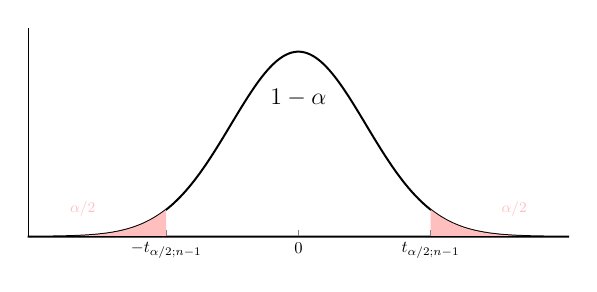
\begin{tikzpicture}[scale = 0.6]
  \begin{axis}[
    no markers,
    domain=-4:4,
    samples=200,
    axis lines*=left,
    ymin=0, ymax=0.45,
    xtick={-1.96, 0, 1.96},
    xticklabels={$-t_{\alpha/2;n-1}$, $0$, $t_{\alpha/2;n-1}$},
    ytick=\empty,
    enlargelimits=false,
    clip=false,
    axis on top,
    width=13cm,
    height=6cm
  ]

  % Courbe normale standard
  \addplot[very thick, black] {exp(-x^2/2)/sqrt(2*pi)} \closedcycle;

  % Remplissage à gauche
  \addplot [
    domain=-4:-1.96,
    samples=100,
    fill=pink,
    draw=none
  ] {exp(-x^2/2)/sqrt(2*pi)} \closedcycle;

  % Remplissage à droite
  \addplot [
    domain=1.96:4,
    samples=100,
    fill=pink,
    draw=none
  ] {exp(-x^2/2)/sqrt(2*pi)} \closedcycle;

  % Texte 1 - alpha
  \node at (axis cs:0,0.3) {\Large $1 - \alpha$};

  % Texte alpha/2 à gauche
  \node at (axis cs:-3.2,0.06) [pink] {\small $\alpha/2$};

  % Texte alpha/2 à droite
  \node at (axis cs:3.2,0.06) [pink] {\small $\alpha/2$};

  \end{axis}
\end{tikzpicture}
    
\end{center}

\end{frame}

\begin{frame}[t]
 \frametitle{Cas 2 pour $\mu$: loi normale, variance inconnue}

 \begin{itemize} \itemsep3mm
\item On cherche $[C_1, C_2]$ tels que $P(C_1\le \alert{\mu} \le C_2)=1-\alpha$
\item On sait que $P\left(\,-t_{\alpha/2;\, n-1}\;\le \;\dfrac{\overline X - \mu}{S/\sqrt{n}}\;\le \;t_{\alpha/2;\, n-1}\,\right)=1-\alpha$
\end{itemize}

%$\frac{\bar{X}-\mu}{S/\sqrt{n}}\sim t_{n-1}\Rightarrow$
\end{frame}

\begin{frame}[t]
 \frametitle{Exemple 2}
 Retournons à l'exemple des disques. Supposons que $\sigma^2$ n'était pas
 connue et qu'on l'estime par la variance échantil\-lonnale des 9 diamètres observés, soit $s^2= 0,0009 \;\text{cm}^2$.

 \vspace{3mm}

 Donnez un intervalle de confiance à 95\% pour $\mu$. Comparez-le avec l'intervalle obtenu en supposant la variance connue.
\end{frame}

\subsection{Loi de $X_1,\ldots,X_n$ inconnue, mais $n$ grand}

\begin{frame}[t]
 \frametitle{Cas 3 pour $\mu$: loi inconnue, n grand}

 \begin{itemize} \itemsep3mm
\item {\color{blue}{On suppose que $X_1,\ldots,X_n$ sont i.i.d. d'une loi inconnue. }}% et $\mu$ est le paramètre d'intér\^et.
\item  Peut-on construire des intervalles de confiance?

 \item L'idée: utiliser le \alert{théorème  central limite } et le fait  que pour $n$ grand :%(dans la pratique on recommande $n\ge 30$):

 \vspace{4mm}
  $s^2\simeq \sigma^2$ et $\overline{X}\approx \mathcal{N}(\mu,s^2/n)\Rightarrow$
\vspace{1cm}
\item 
 Si $n$ est grand, on peut construire des intervalles de confiance dont le niveau sera \alert{approximativement}  du niveau désiré.
\end{itemize}

{\small
Notez qu'il est possible qu'on soit dans une situation où $\sigma^2$ est supposée connue. Il faut donc simplement utiliser $\sigma$ à la place de $s$ dans tout ce qui suit.}
\end{frame}

\begin{frame}[t]
 \frametitle{Cas 3 pour $\mu$: loi inconnue, n grand}

 \begin{itemize} \itemsep3mm
\item On cherche $[C_1, C_2]$ tels que $P(C_1\le \alert{\mu} \le C_2)=1-\alpha$
\item On sait que $P\left(\,-z_{\alpha/2 }\;\le \;\dfrac{\overline X - \mu}{S/\sqrt{n}}\;\le \;z_{\alpha/2 }\,\right)\alert{\approx} 1-\alpha$
    \vspace{7mm}
\item On déduit que $P\left(\overline X \,-\,z_{\alpha/2 } \dfrac{S}{\sqrt{n}}\;\le \;  \mu\;\le \overline X \,+\,z_{\alpha/2 }\dfrac{S}{\sqrt{n}}\,\right)\alert{\approx} 1-\alpha$
\end{itemize}
% $s^2\simeq \sigma^2$ et $\bar{X}\approx \mathcal{N}(\mu,s^2/n)\Rightarrow$
\end{frame}

\begin{frame}[t]
 \frametitle{Exemple 3}

 {\small
 Pour estimer le salaire moyen annuel de jeunes diplômés dans un certain domaine, on  a prélevé un échantillon de taille $n = 100$ et obtenu  $\overline{x}=34~224\,\$$ et $s=4~668\,\$$.\\

 Donnez un intervalle de confiance de niveau 90\% pour le salaire moyen annuel des  jeunes diplômés dans ce domaine.}



\end{frame}


\begin{frame}[t]{La marge d'erreur et l'erreur-type}
Les trois intervalles de confiance pour $\mu$ sont symétriques:

% leur marge d'erreur est donc égale à leur demi-longueur.
$$\begin{array}{cccc}
\overline X &\pm & \multicolumn{2}{c}{\alert{\text{marge d'erreur}}}\\[6mm]
\overline X &\pm & \text{quantile}\;\times&\text{\color{green}{erreur-type}}
\end{array}$$

\vspace{3cm}
{\color{blue}{Longueur}} de l'intervalle$ = 2\times $ marge d'erreur

\end{frame}




\begin{frame}[t]{ }

\centerline{\LARGE\bf \alert{QUIZ !}}
\bigskip
Déterminez si les énoncés suivants sont vrais ou faux.
\vspace{0.3cm}

La marge d'erreur d'un IC sur la moyenne $\mu$ augmente \\(donc la précision diminue) si:
\vspace{0.3cm}

\begin{itemize}\itemsep1cm
  \item la variabilité des mesures augmente.
  \item la taille d'échantillon augmente.
  \item le niveau de confiance augmente.
\end{itemize}

\end{frame}

%%%%%%%%%%%%%%%%%%%%%%%%%%%%%%%%%%%%%%%%%%%%%%%%%%%%%%%%%%%%%%%%%%%%%%%%%%%%%%%%%%%%%%%%%%%%%%%%%%%%%%%%%%%%%%%%%%%%%%%%%%%

\section[IC pour une variance]{Intervalles de confiance pour une variance}

\subsection{Loi normale}

\begin{frame}[t]
 \frametitle{Cas 4 pour $\sigma^2$: loi normale, $\mu$ et $\sigma^2$ inconnues}


 \begin{itemize} \itemsep1mm
\item {\color{blue}{On suppose que $X_1,\ldots,X_n$ i.i.d. loi $\mathcal{N}(\mu,\sigma^2)$, \\
o\`u $\mu$ et $\sigma^2$ sont inconnues}.}% et $\mu$ est le paramètre d'intér\^et.
\item On sait que  $\displaystyle U=\frac{(n-1)\,S^2}{\sigma^2}\;\sim\;\chi^2_{n-1}$
\item Soit $\chi^2_{\alpha/2;\,n-1}$, la valeur telle que $P(U>\chi^2_{\alpha/2;\,n-1})=\alpha/2$. Ainsi,\\
\end{itemize}


\begin{center}
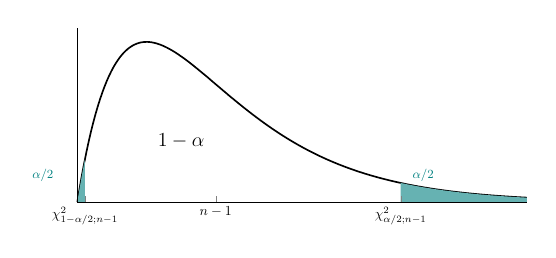
\begin{tikzpicture}[scale = 0.5]
  \begin{axis}[
    no markers,
    domain=0:13,
    samples=200,
    axis lines*=left,
    ymin=0, ymax=0.2,
    xlabel={ },
    ylabel={ },
    xtick={0.22, 4, 9.35},
    xticklabels={$\chi^2_{1-\alpha/2;n-1}$, $n-1$, $\chi^2_{\alpha/2;n-1}$},
    ytick=\empty,
    enlargelimits=false,
    clip=false,
    axis on top,
    width=13cm,
    height=6cm,
  ]

  % Densité de chi carré à 10 degrés de liberté
  \addplot[very thick, black, domain=0:13]
    {x * exp(-x/2) / (4 )};

  % Zone de rejet (alpha à droite)
  \addplot [
    domain=9.35:13,
    samples=100,
    fill=teal!60,
    draw=none
  ]
  {x * exp(-x/2) / (4 )} \closedcycle;
  
    % Zone de rejet (alpha à gauche)
  \addplot [
    domain=0:0.22,
    samples=100,
    fill=teal!60,
    draw=none
  ]
  {x * exp(-x/2) / (4 )} \closedcycle;

  % Texte dans la zone centrale
  \node at (axis cs:3,0.07) {\Large $1 - \alpha$};

  % Texte alpha à droite
  \node at (axis cs:10,0.03) [teal] {\small $\alpha/2$};

    % Texte alpha à gauche
  \node at (axis cs:-1,0.03) [teal] {\small $\alpha/2$};

  \end{axis}
\end{tikzpicture}
\end{center}

\begin{minipage}[b]{6.1cm}{
$P(\chi^2_{1-\alpha/2;\,n-1}\le U\le \chi^2_{\alpha/2;\,n-1})=1-\alpha$.

\vspace{1cm}}
\end{minipage}\end{frame}

\begin{frame}[t]
 \frametitle{Cas 4 pour $\sigma^2$: loi normale, $\mu$ et $\sigma^2$ inconnues}

 \begin{itemize} \itemsep3mm
\item On cherche $[C_1, C_2]$ tels que $P(C_1\le \alert{\sigma^2} \le C_2)=1-\alpha$
\item On sait que $P\left(\chi^2_{1-\alpha/2;\,n-1}\le \dfrac{(n-1)\,S^2}{\sigma^2}\le \chi^2_{\alpha/2;\,n-1}\right)=1-\alpha$
\end{itemize}

% {\small  On cherche deux v.a. $C_1$ et $C_2$ telles que $P[C_1\le\sigma^2\le C_2]=1-\alpha$. On sait  que $\frac{(n-1)S^2}{\sigma^2}\sim\chi^2_{n-1}\Rightarrow$}

\end{frame}

\begin{frame}[t]
 \frametitle{Intervalle pour l'écart-type $\sigma$}

  $P\left(C_1\le \sigma^2\le C_2\right)=1- \alpha $
  \bigskip

  est équivalent à
    \bigskip

  $P\left(\sqrt{C_1}\le \sqrt{\sigma^2}\le\sqrt{C_2}\right)=1 - \alpha $.
    \bigskip

  Pour avoir un IC($\sigma$), on prend la racine carrée des bornes de IC($\sigma^2$).

\end{frame}

\begin{frame}[t]
 \frametitle{Exemple 4}

 {\small
 On veut calibrer la machine qui fabrique les disques de frein pour qu'elle soit le plus stable possible. On veut d'abord estimer la variation du diamètre des disques produits, avec un intervalle de confiance  à 95\%.\\

 Un échantillon de taille 25  a donné une variance échantillonnale de $0,015$ cm$^2$.  On suppose que les diamètres sont i.i.d. de loi normale.}

\end{frame}

\begin{frame}[t]{En extra}
    Seriez-vous capable de construire un intervalle de confiance pour un ratio de variances?
\end{frame}
\begin{frame}[t]{Réponses aux exemples}

{\scriptsize

\begin{enumerate}
  \item
      \begin{itemize}
      \item[b)] {\scriptsize IC($\mu$) à 95\%: $[12,030;\,12,070]$}
      \item[c)] {\scriptsize $n=35$}
     \end{itemize}
 \item IC($\mu$) à 95\%: $[12,028;\,12,072]$
 \item IC($\mu$) à 90\%: $[33\, 456,114 ; \, 34\, 991,886 ]$
 \item IC($\sigma$)à 95\%: $[0,096; \, 0,170]$
 \end{enumerate}
 }
\end{frame}


\end{document}